%%%%%%%%%%%%%%%%%%%%%%%%%%%%%%%%%%%%%%%%%%%%%%%%%%%%%%%%%%%%%%%%%%%%%%%%%%%%%%%%
% TUM-Vorlage: Präsentation
%%%%%%%%%%%%%%%%%%%%%%%%%%%%%%%%%%%%%%%%%%%%%%%%%%%%%%%%%%%%%%%%%%%%%%%%%%%%%%%%
%
% Rechteinhaber:
%     Technische Universität München
%     https://www.tum.de
%
% Gestaltung:
%     ediundsepp Gestaltungsgesellschaft, München
%     http://www.ediundsepp.de
%
% Technische Umsetzung:
%     eWorks GmbH, Frankfurt am Main
%     http://www.eworks.de
%
%%%%%%%%%%%%%%%%%%%%%%%%%%%%%%%%%%%%%%%%%%%%%%%%%%%%%%%%%%%%%%%%%%%%%%%%%%%%%%%%


%%%%%%%%%%%%%%%%%%%%%%%%%%%%%%%%%%%%%%%%%%%%%%%%%%%%%%%%%%%%%%%%%%%%%%%%%%%%%%%%
% Zur Wahl des Seitenverhältnisses bitte einen der beiden folgenden Befehle
% auskommentieren und den ausführen lassen:
%\documentclass[aspectratio=169]{beamer}
\documentclass[notes,t,aspectratio=169]{beamer}
\usepackage[
    orientation=landscape,
    size=custom,
    width=25.4,
    height=14.2875,
    scale=0.5
]{beamerposter}

% Display Notes for pympress
\usepackage{pgfpages}
\setbeameroption{show notes on second screen=right}
\setbeamertemplate{note page}[plain]
\setbeamerfont{note page}{size=\Large}

\newcommand{\PraesentationSchriftgroesseSehrGross}{\fontsize{25}{38}}
\newcommand{\PraesentationSchriftgroesseGross}{\fontsize{18}{27}}
\newcommand{\PraesentationSchriftgroesseNormal}{\fontsize{14}{21}}
\newcommand{\PraesentationSchriftgroesseKlein}{\fontsize{11}{17}}
\newcommand{\PraesentationSchriftgroesseDreizeiler}{\fontsize{7}{10}}
\newcommand{\PraesentationSchriftgroesseAufzaehlungszeichen}{\fontsize{10}{8}}

\newcommand{\PraesentationAbstandAbsatz}{18pt}
\newcommand{\PraesentationPositionKorrekturOben}{-1cm}
\newcommand{\PraesentationBeispieleSchriftgroessen}{25 | 18 | 14 | 11}
\usepackage[utf8]{inputenc}
\usepackage[T1]{fontenc} % Zeichensatzkodierung

\usepackage{calc} % Berechnungen

\usepackage[ngerman]{babel} % Deutsche Lokalisierung
\usepackage{graphicx} % Grafiken
\usepackage[absolute, overlay]{textpos} % Positionierung

% Silbentrennung:
\usepackage{hyphenat}
%\tolerance 2414
%\hbadness 2414
%\emergencystretch 1.5em
%\hfuzz 0.3pt
%\widowpenalty=10000     % Hurenkinder
%\clubpenalty=10000      % Schusterjungen
%\vfuzz \hfuzz

% Euro-Symbol:
\usepackage[gen]{eurosym}
\DeclareUnicodeCharacter{20AC}{\euro{}}

% Schriftart Helvetica:
\usepackage[scaled]{helvet}
\renewcommand{\familydefault}{\sfdefault}

\usepackage{mathptmx} % skalierbare Formelschriften

\usepackage{tabularx}

\usepackage{multicol} % mehrspaltiger Text

\usepackage{tikz}
\usetikzlibrary{arrows, shapes, shapes.multipart, trees, positioning,
    backgrounds, fit, matrix, external, overlay-beamer-styles}

% Diagramme:
\usepackage{pgfplots}
\pgfplotsset{compat=default}

% Erweiterbare Fusszeile:
\newcommand{\PraesentationFusszeileZusatz}{}

\usepackage{bookmark} % Lesezeichen

% Unterdrückung layoutbedingter Warnungen
\usepackage[immediate]{silence}
\WarningFilter[layout]{lastpage}{Rerun to get the references right} % Gesamtseitenzahl
\WarningFilter[layout]{latex}{Label(s) may have changed.} % Referenz auf letzte Seite
\WarningFilter[layout]{pgfplots}{running in backwards compatibility mode (unsuitable tick labels; missing features).} % Labelerstellung ab Version 1.17 nicht abwärtskompatibel
\WarningFilter[layout]{latex}{There were undefined references}
\WarningFilter[layout]{latex}{Reference `PraesentationDiagramm} % Erstellung einer Legende außerhalb des Diagrammbereichs

% Debugging:
%\DeactivateWarningFilters[layout] % Unterdrückte Warnungen einschalten
\usepackage{listings}

\lstdefinelanguage{rv64}{
    morekeywords={
        addi, bne,
        a1, x0
    },
    sensitive=false
}

\definecolor{SbtComment}{RGB}{80, 80, 80}

\lstdefinelanguage{SbtIr}{
    morekeywords={
        block,
        i64, i32, i16, i8, imm,
        immediate, add,
        cjump, jump
    },
    morecomment=[l]{//},
    morecomment=[s]{/*}{*/}
}

\usepackage[verbatim]{lstfiracode}
\lstset{
    style=FiraCodeStyle, % Use predefined FiraCodeStyle
    basicstyle=\ttfamily, % Use \ttfamily for source code listings
    keywordstyle=\color{TUMBlauDunkel},
    commentstyle=\color{SbtComment}
}

 % Seitenverhältnis 16:9
%%%%%%%%%%%%%%%%%%%%%%%%%%%%%%%%%%%%%%%%%%%%%%%%%%%%%%%%%%%%%%%%%%%%%%%%%%%%%%%%


%%%%%%%%%%%%%%%%%%%%%%%%%%%%%%%%%%%%%%%%%%%%%%%%%%%%%%%%%%%%%%%%%%%%%%%%%%%%%%%%
%%%%%%%%%%%%%%%%%%%%%%%%%%%%%%%%%%%%%%%%%%%%%%%%%%%%%%%%%%%%%%%%%%%%%%%%%%%%%%%%
% TUM-Vorlage: Personenspezifische Informationen
%%%%%%%%%%%%%%%%%%%%%%%%%%%%%%%%%%%%%%%%%%%%%%%%%%%%%%%%%%%%%%%%%%%%%%%%%%%%%%%%
%
% Rechteinhaber:
%     Technische Universität München
%     https://www.tum.de
% 
% Gestaltung:
%     ediundsepp Gestaltungsgesellschaft, München
%     http://www.ediundsepp.de
% 
% Technische Umsetzung:
%     eWorks GmbH, Frankfurt am Main
%     http://www.eworks.de
%
%%%%%%%%%%%%%%%%%%%%%%%%%%%%%%%%%%%%%%%%%%%%%%%%%%%%%%%%%%%%%%%%%%%%%%%%%%%%%%%%

% Für die Person anpassen:

% Allgemein:
\newcommand{\AllgemeinGestalter}{ediundsepp Gestaltungsgesellschaft}
\newcommand{\AllgemeinErsteller}{eWorks GmbH}

% Universität:
\newcommand{\UniversitaetName}{Technische Universität München}
\newcommand{\UniversitaetAbkuerzung}{TUM}
\newcommand{\UniversitaetWebseite}{www.tum.de}
\newcommand{\UniversitaetLogoBreite}{19mm}
\newcommand{\UniversitaetLogoHoehe}{1cm}

\newcommand{\UniversitaetAdresse}{%
	Arcisstraße~21\\%
	80333~München%
}

\hyphenation{} % eigene Silbentrennung
                    % !!! DATEI ANPASSEN !!!
%%%%%%%%%%%%%%%%%%%%%%%%%%%%%%%%%%%%%%%%%%%%%%%%%%%%%%%%%%%%%%%%%%%%%%%%%%%%%%%%

\newcommand{\Datum}{\today}

\renewcommand{\PraesentationFusszeileZusatz}{Rechnerarchitektur-Großpraktikum 2021 | Statische Binärübersetzung von RISC-V in x86-64}

\title{Statische Binärübersetzung von RISC-V in x86-64}
\author{Lukas Döllerer, Jonathan Hettwer, Johannes Maier, Tobias Schwarz, Felix Solcher}
\institute[]{Rechnerarchitektur-Großpraktikum 2021}
\date[\Datum]{Garching, 16. Juli 2021}
\subject{Statische Binärübersetzung von RISC-V in x86-64}


%%%%%%%%%%%%%%%%%%%%%%%%%%%%%%%%%%%%%%%%%%%%%%%%%%%%%%%%%%%%%%%%%%%%%%%%%%%%%%%%
%%%%%%%%%%%%%%%%%%%%%%%%%%%%%%%%%%%%%%%%%%%%%%%%%%%%%%%%%%%%%%%%%%%%%%%%%%%%%%%%
% EINSTELLUNGEN
%%%%%%%%%%%%%%%%%%%%%%%%%%%%%%%%%%%%%%%%%%%%%%%%%%%%%%%%%%%%%%%%%%%%%%%%%%%%%%%%

\newcommand{\PraesentationSeitenrand}{8.9mm}
\newcommand\crule[3][black]{\textcolor{#1}{\rule{#2}{#3}}}

\newlength\smallerbaselineskip
\setlength{\smallerbaselineskip}{0.8\baselineskip}

    % Blautöne:
\definecolor{TUMBlau}{RGB}{0,101,189} % Pantone 300
\definecolor{TUMBlauDunkel}{RGB}{0,82,147} % Pantone 301
\definecolor{TUMBlauHell}{RGB}{152,198,234} % Pantone 283
\definecolor{TUMBlauMittel}{RGB}{100,160,200} % Pantone 542

    % Hervorhebung:
\definecolor{TUMElfenbein}{RGB}{218,215,203} % Pantone 7527 -Elfenbein
\definecolor{TUMGruen}{RGB}{162,173,0} % Pantone 383 - Grün
\definecolor{TUMOrange}{RGB}{227,114,34} % Pantone 158 - Orange
\definecolor{TUMGrau}{gray}{0.6} % Grau 60%


\setbeamercolor*{alerted text}{fg=TUMOrange}

\newcommand{\PraesentationSetzeTextfarbe}{
    \color{PraesentationTextfarbe}
    \setbeamercolor*{frametitle}{fg=PraesentationTextfarbe}
    \setbeamercolor*{normal text}{fg=PraesentationTextfarbe}
    \setbeamercolor{itemize/enumerate body}{fg=PraesentationTextfarbe}
    \setbeamercolor*{itemize item}{fg=PraesentationTextfarbe}
}

\newcommand{\PraesentationFarbschemaStandard}{
    \setbeamercolor*{background canvas}{}
    \definecolor{PraesentationTextfarbe}{rgb}{0,0,0}
    \PraesentationSetzeTextfarbe
}

\newcommand{\PraesentationFarbschemaWeissBlau}{
    \setbeamercolor*{background canvas}{bg=TUMBlauDunkel}
    \definecolor{PraesentationTextfarbe}{rgb}{1,1,1}
    \PraesentationSetzeTextfarbe
}

\newcommand{\PraesentationFarbschemaWeissSchwarz}{
    \setbeamercolor*{background canvas}{bg=black}
    \definecolor{PraesentationTextfarbe}{rgb}{1,1,1}
    \PraesentationSetzeTextfarbe
}

\newcommand{\PraesentationTitelseiteInhalt}{
    \begin{textblock*}{\paperwidth}[0,0](0cm,-\PraesentationSeitenrand - 6.5mm + \PraesentationPositionKorrekturOben)%
        \color{PraesentationTextfarbe}%
        \frametitle{\inserttitle}
        \vspace*{49.4mm}
        \usebeamerfont{author}\selectfont\insertauthor\\
	    \vspace*{2mm}
        \insertinstitute\\
        \insertdate%
    \end{textblock*}
}

\newcommand{\PraesentationSeitenkopfInhalt}[1]{
    %\vspace*{31.7mm}%
    \begin{textblock*}{1.68cm}[1,0](\paperwidth - \PraesentationSeitenrand - \PraesentationSeitenrand, 0cm)%
        \includegraphics[width=1.68cm]{#1}%
    \end{textblock*}
    \begin{textblock*}{3cm}[1,0](\paperwidth - \PraesentationSeitenrand, -\PraesentationSeitenrand)%
        \hbox{%
            \color{PraesentationTextfarbe}
            \hbox{\insertframenavigationsymbol}%
            \hbox{\insertsubsectionnavigationsymbol}%
            \hbox{\insertsectionnavigationsymbol}%
        }%
    \end{textblock*}%
}

\newcommand{\PraesentationBildUhrenturm}{%
    \begin{textblock*}{10.82cm}[1,1](\paperwidth - \PraesentationSeitenrand - \PraesentationSeitenrand, \paperheight - 9mm)%
        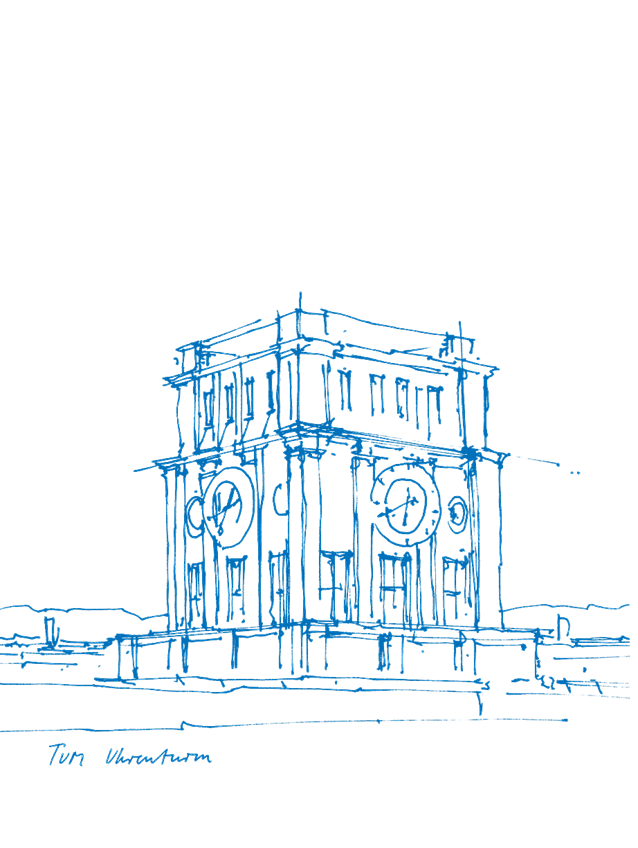
\includegraphics{img/TUM_Uhrenturm.png}%
    \end{textblock*}%
}

\newcommand{\PraesentationStartseiteUhrenturm}{
    \setbeamertemplate{title page}{%
        \PraesentationSeitenkopfInhalt{img/Universitaet_Logo_RGB.pdf}
        \PraesentationBildUhrenturm
        \PraesentationTitelseiteInhalt
    }
}

\newcommand{\PraesentationStartseiteLeer}{
    \setbeamertemplate{title page}{%
        \PraesentationSeitenkopfInhalt{img/Universitaet_Logo_weiss.pdf}
        \PraesentationTitelseiteInhalt
    }
}


\newcommand{\PraesentationMasterStandard}{
    \PraesentationFarbschemaStandard

    \PraesentationStartseiteUhrenturm

    \setbeamertemplate{headline}{
        \PraesentationSeitenkopfInhalt{img/Universitaet_Logo_RGB.pdf}
    }
}

\newcommand{\PraesentationMasterWeissBlau}{
    \PraesentationFarbschemaWeissBlau

    \PraesentationStartseiteLeer

    \setbeamertemplate{headline}{
        \PraesentationSeitenkopfInhalt{img/Universitaet_Logo_weiss.pdf}
    }
}

\newcommand{\PraesentationMasterKopfzeileDreizeiler}{
    \PraesentationFarbschemaStandard

    \setbeamertemplate{title page}{%
        \PraesentationBildUhrenturm
        \begin{textblock*}{\paperwidth}[0,0](0cm, -7.8mm)%
            \color{TUMBlau}\PraesentationSchriftgroesseDreizeiler\selectfont%
            \LehrstuhlName\\%
            \FakultaetName\\%
            \UniversitaetName\\%
            \normalcolor\normalsize\selectfont%
        \end{textblock*}%
        \PraesentationSeitenkopfInhalt{img/Universitaet_Logo_RGB.pdf}
        \PraesentationTitelseiteInhalt
    }

    \setbeamertemplate{headline}{
        \begin{textblock*}{\paperwidth}[0,0](0cm, -7.8mm)%
            \color{TUMBlau}\PraesentationSchriftgroesseDreizeiler\selectfont%
            \LehrstuhlName\\%
            \FakultaetName\\%
            \UniversitaetName\\%
            \normalcolor\normalsize\selectfont%
        \end{textblock*}%
        \PraesentationSeitenkopfInhalt{img/Universitaet_Logo_RGB.pdf}
    }
}

\newcommand{\PraesentationMasterWeissSchwarz}{
    \PraesentationFarbschemaWeissSchwarz

    \setbeamertemplate{title page}{%
        \PraesentationTitelseiteInhalt
        \PraesentationSeitenkopfInhalt{img/Universitaet_Logo_weiss.pdf}
    }

    \setbeamertemplate{headline}{
        \PraesentationSeitenkopfInhalt{img/Universitaet_Logo_weiss.pdf}
    }
}

\newcommand{\PraesentationTitelseite}{\frame[plain]{\titlepage}}
\newcommand{\PraesentationUeberschriftZweizeilig}[2]{\frametitle{#1\\[8mm]#2}}

\setbeamersize{
    text margin left=\PraesentationSeitenrand,
    text margin right=\PraesentationSeitenrand
}

\setbeamertemplate{frametitle}{%
    {\rule{0pt}{42mm + \PraesentationPositionKorrekturOben}\PraesentationSchriftgroesseSehrGross\selectfont\insertframetitle\newline\vspace*{-6.7mm}}%
}

% Aufzählungen:
\newcommand{\PraesentationAufzaehlungEbeneEinsSymbol}{\raise2pt\hbox{\donotcoloroutermaths\usebeamercolor{itemize subitem}\PraesentationSchriftgroesseAufzaehlungszeichen$\bullet$}}
\newcommand{\PraesentationAufzaehlungEbeneZweiSymbol}{\raise1.25pt\hbox{\donotcoloroutermaths\usebeamercolor{itemize subitem}$-$}}
\setbeamertemplate{itemize items}[circle]
\setbeamertemplate{itemize subitem}[triangle]
\setbeamercolor{itemize subitem}{fg=black}
\setbeamerfont{itemize/enumerate subbody}{size=\normalsize}
\setbeamertemplate{itemize item}{\PraesentationAufzaehlungEbeneEinsSymbol}
\setbeamertemplate{itemize subitem}{\PraesentationAufzaehlungEbeneZweiSymbol{}}
%\addtolength{\leftmarginii}{16mm-2pt}%

\newenvironment{PraesentationAufzaehlung}
{%
    \vspace{-\baselineskip}%
    \begin{itemize}%
        \setlength{\itemsep}{0pt}%
        \setlength{\parskip}{0pt}%
        \setlength{\parsep}{0pt}%
        \addtolength{\itemindent}{-1ex}%
}{%
    \end{itemize}%
}

%%%%%%%%%%%%%%%%%%%%%%%%%%%%%%%%%%%%%%%%%%%%%%%%%%%%%%%%%%%%%%%%%%%%%%%%%%%%%%%%
% DOKUMENT
%%%%%%%%%%%%%%%%%%%%%%%%%%%%%%%%%%%%%%%%%%%%%%%%%%%%%%%%%%%%%%%%%%%%%%%%%%%%%%%%


% PDF-Einstellungen:
\hypersetup{
    pdfstartview={Fit},
    pdfproducer={\AllgemeinErsteller},
    pdfcreator={\AllgemeinGestalter}
}

\textblockorigin{\PraesentationSeitenrand}{\PraesentationSeitenrand} % Ursprung für Positionierung

\setbeamerfont{footnote}{size=\PraesentationSchriftgroesseKlein}

\setbeamertemplate{footline}{
    \hbox{%
        \usebeamerfont{footnote}%
        \begin{beamercolorbox}[wd=.9\paperwidth]{}%
            \hspace*{\PraesentationSeitenrand}%
            \PraesentationFusszeileZusatz{}%
        \end{beamercolorbox}%
        \begin{beamercolorbox}[wd=.1\paperwidth]{}%
            \insertframenumber{}%
            \raggedleft
            \hspace*{\PraesentationSeitenrand}%
        \end{beamercolorbox}%
        \vspace*{3.25mm}%
    }%
}

\setbeamertemplate{navigation symbols}{}

\begin{document}
\setlength{\baselineskip}{\PraesentationAbstandAbsatz}
\setlength{\parskip}{\baselineskip}
 % !!! NICHT ENTFERNEN !!!
%%%%%%%%%%%%%%%%%%%%%%%%%%%%%%%%%%%%%%%%%%%%%%%%%%%%%%%%%%%%%%%%%%%%%%%%%%%%%%%%


%%%%%%%%%%%%%%%%%%%%%%%%%%%%%%%%%%%%%%%%%%%%%%%%%%%%%%%%%%%%%%%%%%%%%%%%%%%%%%%%
% FOLIENSTIL: Standard
\PraesentationMasterStandard

\PraesentationTitelseite % Fügt die Startseite ein


% draws an arrow from (#2,#3) to (#2+#4,#3) with height of #5 (arrow in x direction)
% color (and other arguments, like visible on), startX, startY, length (X dir), height (Y dir)
\newcommand{\TikZArrowX}[5]{
    \filldraw[#1] (#2,#3) -- (#2,#3+#5*2/3) -- (#2+#4/2,#3+#5*2/3) -- (#2+#4/2,#3+#5) -- (#2+#4,#3) -- (#2+#4/2,#3-#5) -- (#2+#4/2,#3-#5*2/3) -- (#2,#3-#5*2/3) -- (#2,#3);
    \draw[#1, black] (#2,#3) -- (#2,#3+#5*2/3) -- (#2+#4/2,#3+#5*2/3) -- (#2+#4/2,#3+#5) -- (#2+#4,#3) -- (#2+#4/2,#3-#5) -- (#2+#4/2,#3-#5*2/3) -- (#2,#3-#5*2/3) -- (#2,#3);
}

% draws an arrow from #2,#3) to (#2,#3+#5) with height of #4 (arrow in y direction)
% color (and other arguments, like visible on), startX, startY, length (X dir), height (Y dir), color
\newcommand{\TikZArrowY}[5]{
    \filldraw[#1] (#2,#3) -- (#2+#4*2/3,#3) -- (#2+#4*2/3,#3+#5/2) -- (#2+#4,#3+#5/2) -- (#2,#3+#5) -- (#2-#4,#3+#5/2) -- (#2-#4*2/3,#3+#5/2) -- (#2-#4*2/3,#3) -- (#2,#3);
    \draw[#1, black] (#2,#3) -- (#2+#4*2/3,#3) -- (#2+#4*2/3,#3+#5/2) -- (#2+#4,#3+#5/2) -- (#2,#3+#5) -- (#2-#4,#3+#5/2) -- (#2-#4*2/3,#3+#5/2) -- (#2-#4*2/3,#3) -- (#2,#3);
}

% draws one entry of the color legend for the program scheme
% color, text, posX, posY (left, top coordinate)
\newcommand{\colorLegendEntry}[4]{
    \filldraw[#1] (#3,#4) rectangle (#3+1,#4+1);
    \draw[black] (#3,#4) rectangle (#3+1,#4+1);
    \node at (#3+0.5,#4+0.4) (color_legend_entry_point) {};
    \node[right=2mm of color_legend_entry_point] (color_legend_entry_text) {#2};
}

% draws a color legend for the program scheme
% posX, posY (left, top coordinate)
\newcommand{\colorLegend}[2] {
    \colorLegendEntry{TUMOrange}{Static Translator Parts}{#1}{#2}
    \colorLegendEntry{TUMBlauDunkel}{Immediate Representation (IR)}{#1}{#2-1.5}
    \colorLegendEntry{purple}{Maschine Code / ELF File}{#1}{#2-3}
}

% draws the schematic presentation of the program
% scale, fontSize
\newcommand{\ProgramSchemeVersionOne}[2]{
    \begin{center}
        \begin{tikzpicture}[very thick, scale=#1]
            % draw color legend
            \colorLegend{-2}{-6}

            % riscv elf file rectangle
            % background
            \filldraw[purple, visible on=<2->] (-2,-2) rectangle (2,2);
            % black border
            \draw[black, visible on=<2->] (-2,-2) rectangle (2,2);
            % label
            \node[align=center, visible on=<2->] at (0,0) (riscv_text) {\fontsize{#2}{#2} \selectfont RISC-V};

            % lifter arrow
            \TikZArrowX{TUMOrange, visible on=<3->}{2}{0}{6}{1.5}
            % arrow label
            \node[align=center, visible on=<3->] at (4.5,0) (lifter_text) {\fontsize{#2}{#2} \selectfont Lifter};

            % ir (unoptimized) rectangle
            % background
            \filldraw[TUMBlauDunkel, visible on=<4->] (8,-2) rectangle (12,2);
            % black border
            \draw[black, visible on=<4->] (8,-2) rectangle (12,2);
            % label
            \node[align=center, visible on=<4->] at (10,0) (ir_text_1) {\fontsize{#2}{#2} \selectfont IR};

            % optimizer arrow
            \TikZArrowX{TUMOrange, visible on=<5->}{12}{0}{6}{1.5}
            % arrow label
            \node[align=center, visible on=<5->] at (14.5,0) (optimizer_text) {\fontsize{#2}{#2} \selectfont Optimizer};

            % ir (optimized) rectangle
            % background
            \filldraw[TUMBlauDunkel, visible on=<6->] (18,-2) rectangle (22,2);
            % black border
            \draw[black, visible on=<6->] (18,-2) rectangle (22, 2);
            % label
            \node[align=center, visible on=<6->] at (20,0) (ir_text_2) {\fontsize{#2}{#2} \selectfont IR};

            % compiler arrow
            \TikZArrowX{TUMOrange, visible on=<7->}{22}{0}{6}{1.5}
            % arrow label
            \node[align=center, visible on=<7->] at (24.5,0) (compiler_text) {\fontsize{#2}{#2} \selectfont Compiler};

            % x86_64 rectangle
            %background
            \filldraw[purple, visible on=<8->] (28,-2) rectangle (32,2);
            % black border
            \draw[black, visible on=<8->] (28,-2) rectangle (32,2);
            % label
            \node[align=center, visible on=<8->] at (30,0) (x86_64_text) {\fontsize{#2}{#2} \selectfont x86\_64};
        \end{tikzpicture}
    \end{center}
}


\begin{frame}
    \frametitle{Programmübersicht}
    %alignment to have some space between headline an the schematic
    ~\\
    ~\\
    \ProgramSchemeVersionOne{0.6}{18}
\end{frame}

%%%%%%%%%%%%%%%%%%%%%
%% IR Aufbau Folie %%
%%%%%%%%%%%%%%%%%%%%%

\begin{frame}
    \frametitle{Intermediate Representation}{Aufbau}
    \pause
    \begin{itemize}
        \item Die IR besteht aus mehreren "`\textbf{Basic Blocks}"'
              \pause
        \item Basic Block: Eine Folge von sequentiellen Instruktionen, beendet durch eine Kontrollflussopertion
              \pause
        \item Ein Basic Block enthält Variablen in SSA-Form und Operationen
              \pause
        \item \textbf{Static single assignment (SSA):} Jeder Variable wird genau einmal ein Wert zugewiesen
              \pause
        \item Ein Basic Block erhält Eingaben in Form von Statics
              \pause
        \item Die Basic Blocks sind durch die Kontrollflussoperationen miteinander verbunden
              \pause
        \item Zur Nachvervolgung von Lese- und Schreiboperationen gibt es Memory Tokens $\rightarrow$ Optimierungen
    \end{itemize}
\end{frame}

\begin{frame}
    \frametitle{Intermediate Representation}{Operationen}
    \pause

    ~\\
    ~\\

    \begin{columns}[c]
        \column{0.4\textwidth}
        Instruktionen:
        \begin{itemize}
            \item Speicher: \texttt{store}, \texttt{load}
            \item Arithmetisch: \texttt{add}, \texttt{sub}, \texttt{mul}, ...
            \item Logisch: \texttt{and}, \texttt{or}, \texttt{shl}, ...
            \item Sonstige: Typkonvertierung, ...
        \end{itemize}

        \pause
        \column{0.4\textwidth}
        Kontrollflussoperationen:
        \begin{itemize}
            \item Sprünge: \texttt{jump}, \texttt{ijump}, \texttt{cjump}
            \item Sprünge (erweitert): \texttt{call}, \texttt{icall}, \texttt{return}
            \item \texttt{unreachable}
            \item \texttt{syscall}
        \end{itemize}
    \end{columns}
\end{frame}

%%%%%%%%%%%%%%
%% IR Folie %%
%%%%%%%%%%%%%%

\begin{frame}[fragile]
    \frametitle{Intermediate Representation}{Beispiel}
    \pause
    ~\\
    ~\\
    ~\\
    \begin{columns}[c]
        \column{0.275 \textwidth}
        \begin{lstlisting}[language=rv64]
        [...]
        addi a1, x0, 100
    loop:
        addi a1, a1, -1
        bne a1, x0, loop
        [...]
        \end{lstlisting}

        \pause
        \column{0.125 \textwidth}
        \begin{tikzpicture}[scale=0.72]
            \TikZArrowX{TUMOrange}{0}{0}{4}{1}
        \end{tikzpicture}

        \pause

        \column{0.6 \textwidth}
        \begin{lstlisting}[language=SbtIr]
block b1(inputs) <= [predecessors] {
    i64 v0 <- @1
    [...] // more statics
    imm v33 <- immediate 0
    imm v34 <- immediate 100
    i64 <- add i64 v33, i64 v33
} => [(jump, [b2, ...])]

block b2(inputs) <= [predecessors] { // loop
    [...] // statics
    imm v33 <- immediate -1
    i64 v34 <- add i64 v11, i64 v33
} => [(cjump, [b2, ...]), (jump, [...])]
    \end{lstlisting}
    \end{columns}

\end{frame}
\clearpage

%%%%%%%%%%%%%%%%%%%%%%%%%%%
%% ELF File Parser Folie %%
%%%%%%%%%%%%%%%%%%%%%%%%%%%

\begin{frame}[fragile]
    \frametitle{Lifter}{ELF Binärdatei laden und Instruktionsbytes decodieren}
    \begin{columns}[c]
        \column{0.5 \textwidth}
        \begin{enumerate}
            \visible<2-> {
            \item ELF File prüfen.
                  }
                  \visible<3-> {
            \item Program Header, Sections und Symbole auslesen.
                  \visible<4-> {
            \item Section Bytes $\rightarrow$ Instruktionen durch \textbf{frvdec} decodieren.
                  }
        \end{enumerate}
        }
        \column{0.50 \textwidth}
        \begin{lstlisting}[basicstyle=\footnotesize, breaklines=true, escapeinside={@@}]
ELF Header:
    Magic:   7f 45 4c 46 02 01 01 00 00 00 00 00 00 00 00 00
    Class:                             @\textcolor{TUMBlauDunkel}{ELF64}@
    Data:                              @\textcolor{TUMBlauDunkel}{2's complement, little endian}@
    Version:                           1 (current)
    OS/ABI:                            UNIX - @\textcolor{TUMBlauDunkel}{System V}@
    ABI Version:                       0
    Type:                              @\textcolor{TUMBlauDunkel}{EXEC}@ (Executable file)
    Machine:                           @\textcolor{TUMBlauDunkel}{RISC-V}@
    Version:                           0x1
    Entry point address:               @\textcolor{TUMBlauDunkel}{0x100b0}@
    Start of program headers:          64 (bytes into file)
    Start of section headers:          688 (bytes into file)
    Flags:                             0x5, RVC, double-float ABI
    Size of this header:               64 (bytes)
    Size of program headers:           56 (bytes)
    Number of program headers:         2
    Size of section headers:           64 (bytes)
    Number of section headers:         6
    Section header string table index: 5
        \end{lstlisting}
    \end{columns}
\end{frame}
\clearpage

\note[itemize]{
    \item ELF Prüfung: Prüfbits, System-V ABI, 64-Bit, Little Endian, RISC-V Machine
    \item Symbole weren bei gestrippten ELF-Binaries nicht eingelesen
    \item 32-Byte bzw. 16-Byte Compressed mit frvdec decodieren
}

%%%%%%%%%%%%%%%%%%%%%%%%%%
%% Lifter General Folie %%
%%%%%%%%%%%%%%%%%%%%%%%%%%

\begin{frame}
    \frametitle{Lifter}{RISC-V Instruktionen in IR Code umwandeln}
    \begin{enumerate}
        \setlength\itemsep{0.6em}
        \item Instruktionen sequenziell lesen:
              \pause
              \vspace{0.5em}
              \begin{enumerate}
                  \setlength\itemsep{0.6em}
                  \item Instruktionen in IR parsen
                        \pause
                  \item Wiederhole bis eine \textbf{Kontrollfluss ändernde Instruktion} auftritt
                        \pause
                  \item Beende Basic Block $\rightarrow$ starte neuen Basic Blöck für jede Kontrollflussänderung
                        \pause
                  \item Starte für jeden \textbf{neuen} Basic Block wieder bei 1
              \end{enumerate}
              \pause
        \item Sollte Schritt 1 nicht alle vorhandenen Instruktionen in Basic Blöcke gepackt haben:\\ Beginne ab erster \textbf{unbetrachteter} Adresse / Instruktion erneut mit Schritt 1
    \end{enumerate}
\end{frame}
\clearpage

\note[itemize]{
    \item Rekursives parsen
    \item Start bei ELF Einstiegspunkt
    \item RISC-V Instruktionen sequentiell in IR Instruktionen übertragen
    \item Kontrollfluss-ändernde Instruktionen beenden Basic Blöcke
    \item Alle möglichen Sprungziele starten neue Basic Blöcke
    \item Diese werden rekursiv weiter geliftet
    \item Am Ende gehen wir über alle nicht-geliftete Adressen und starten neue Basic Blöcke
}

%%%%%%%%%%%%%%%%%%%%%%%%%%%%%%%
%% Lifter CfOps Folie %%
%%%%%%%%%%%%%%%%%%%%%%%%%%%%%%%

\begin{frame}
    \frametitle{Lifter}{Kontrollflussoperationen}
    \pause
    \begin{enumerate}
        \setlength\itemsep{0.5em}
        \item System Calls (\lstinline[columns=fixed]{ecall})
              \begin{itemize}
                  \item Schreibt Rückgabewerte auf Statics
              \end{itemize}
              \pause
        \item Bedingte Sprünge (\lstinline[columns=fixed]{branch})
              \vspace{0.5em}
              \setlength\itemsep{0.6em}
              \begin{itemize}
                  \item Vergleiche: \setlength\itemsep{0.6em}\begin{itemize}
                            \item \lstinline[columns=fixed]{gleich}
                            \item \lstinline[columns=fixed]{signed lower}
                            \item \lstinline[columns=fixed]{unsigned lower}
                        \end{itemize}
                  \item Generiert 2 Kontrollflussoperationen
              \end{itemize}
              \pause
        \item Direkte Sprünge (\lstinline[columns=fixed]{jal})
              \pause
        \item Indirekte Sprünge (\lstinline[columns=fixed]{jalr})
              \begin{itemize}
                  \item Unbekanntes Sprungziel $\rightarrow$ Backtracking
                  \item Backtracking nur zur Kontrollflussbestimmung im Lifter
              \end{itemize}
    \end{enumerate}
\end{frame}
\clearpage

\note[itemize]{

}


%%%%%%%%%%%%%%%%%%%%%
%% Generator Folie %%
%%%%%%%%%%%%%%%%%%%%%

\begin{frame}
    \frametitle{Generator}{Übersetztung der IR zu x86\_64}
    \pause
    \begin{itemize}
        \item Sehr einfache, aber korrekte übersetztung
              \pause
        \item RISC-V Stack wird simuliert % es wird nicht der x86-64 Stack verwendet
              \pause
        \item Indirekte Sprünge werden per Lookup zur Laufzeit aufgelöst
              \pause
        \item RISC-V System-V ABI (Startup, Syscall) zur Laufzeit emuliert
              \pause
        \item Original ELF Programm als binäres Speicherbild an exakter Adresse eingebunden
              \pause
        \item Erste Optimierung: Eliminerung von Redundanzen bei den Statics
    \end{itemize}
\end{frame}
\clearpage

%%%%%%%%%%%%%%%%%%%%%%%%%%%%%%
%% Technische Demonstration %%
%%%%%%%%%%%%%%%%%%%%%%%%%%%%%%

\begin{frame}
    \frametitle{Technische Demonstration}{Demonstration des aktuellen Standes}

    % 4-6 Minuten
    % helloworld, helloworld2, fibonacci
    % besser: irgendein program das mit musl libc compiliert ist (im besten falle gzip)
    % + etwas erklären was da geliftet wurde
    % 1. originales program kurz erklären (was es macht, wie es gebaut wurde, andere besonderheiten)
    % 2. originales program ausführen
    % 3. translaten
    % 4. translates program ausführen
\end{frame}
\clearpage

%%%%%%%%%%%%%%%%%%%%%%%%%%%%%%%%%%%%%%%%%%%%%%%%%%%%%%%%%%%%%%%%%%%%%%%%%%%%%%%%
\end{document} % !!! NICHT ENTFERNEN !!!
%%%%%%%%%%%%%%%%%%%%%%%%%%%%%%%%%%%%%%%%%%%%%%%%%%%%%%%%%%%%%%%%%%%%%%%%%%%%%%%%
